%proportional corrected algorithm methods
\subsubsection*{Algorithm}
We attempted to correct the dark spot issue by significantly reducing the absolute difference between dark pixels and the average colour, ensuring that the dark spots would instead have colours close to the average. We perform this correction on the output of the proportional adjustment algorithm.

\begin{equation} \label{eq:prop_corr_algo}
  r'' = \left.
  \begin{dcases}
    \displaystyle \mean{r'} - \frac{(\mean{r'} - r')}{\alpha}, & \text{for } r' < \mean{r'} \\
    \displaystyle r', & \text{for } r' \geq \mean{r'} \\
  \end{dcases}
  \right.\\
\end{equation}

\nomenclature{$r''$}{Value of the red channel of the pixel after a second algorithm is applied.}
\nomenclature{$\mean{r'}$}{Average value of the red channel of the hand image outputed by the first algorithm.}

Where $\alpha$ is a constant, $\alpha  > 1$. The same equation applies for the $g$ and $b$ channels.

\subsubsection*{Results}
See Table \ref{tab:prop_correct_test} in Appendix \ref{app:prop_corr_a10}, \ref{app:prop_corr_a5} and \ref{app:prop_corr_a3} for complete results for a range of values for $\alpha$. A portion of the results for $\alpha = 3$ is reproduced here for convenience.

\begin{longtable}{|c||c|c|c|}
    \caption*{Test results of proportional adjusting with correction for dark spots, alpha = 3 from Table \ref{tab:prop_correct_test_a3} in the Appendix \ref{app:prop_corr_a3}}\\
    \hline
    No. & Original & Target & Results \\
    \hline  \ref{row:prop_correct_test_a3_hand_dark_to_hand_brown} &
  \begin{minipage}{.29\textwidth}
    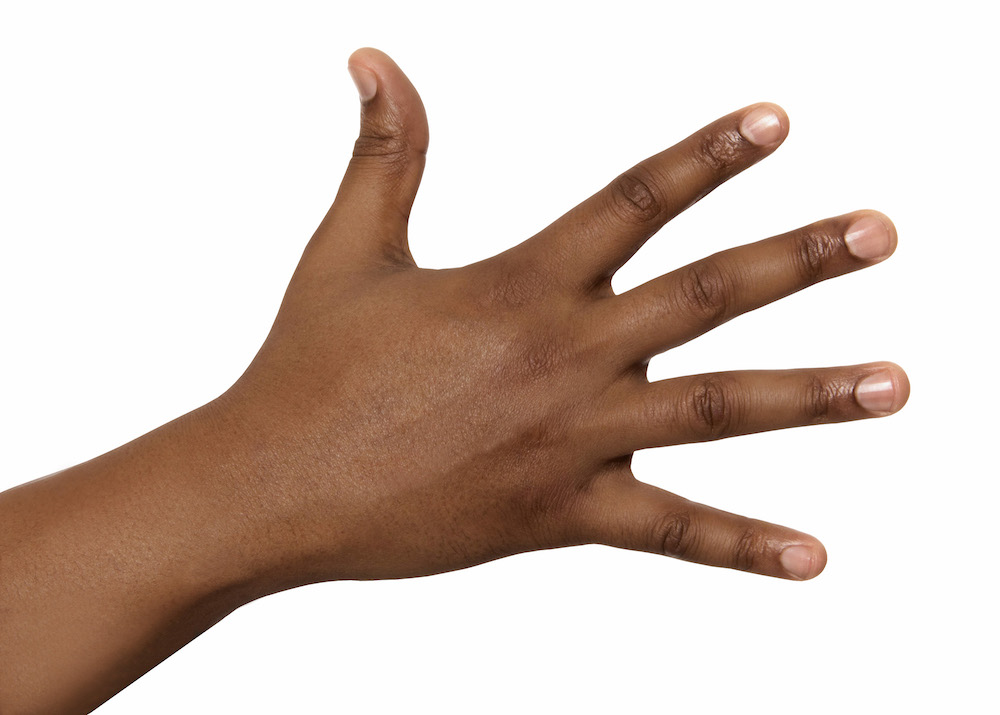
\includegraphics[width=\textwidth,height=\textheight,keepaspectratio]{../inputs/hand_dark.jpg}
  \end{minipage} & 
  \begin{minipage}{.29\textwidth}
    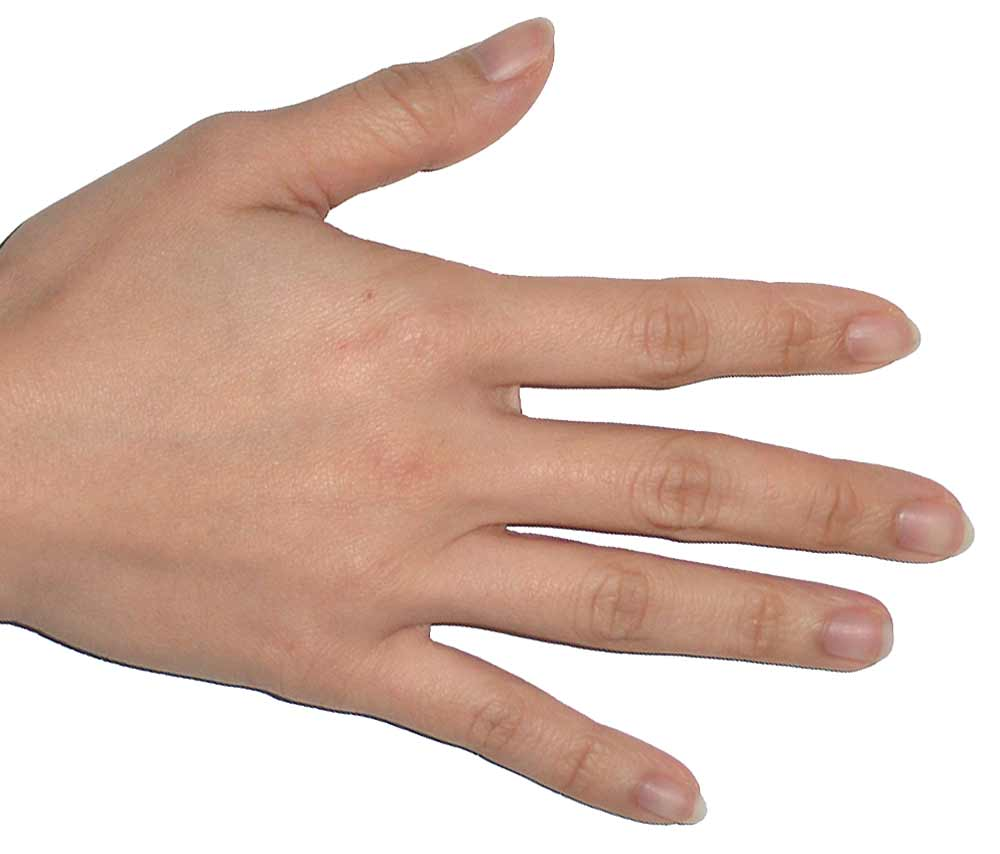
\includegraphics[width=\textwidth,height=\textheight,keepaspectratio]{../inputs/hand_light.jpg}
  \end{minipage} & 
  \begin{minipage}{.29\textwidth}
    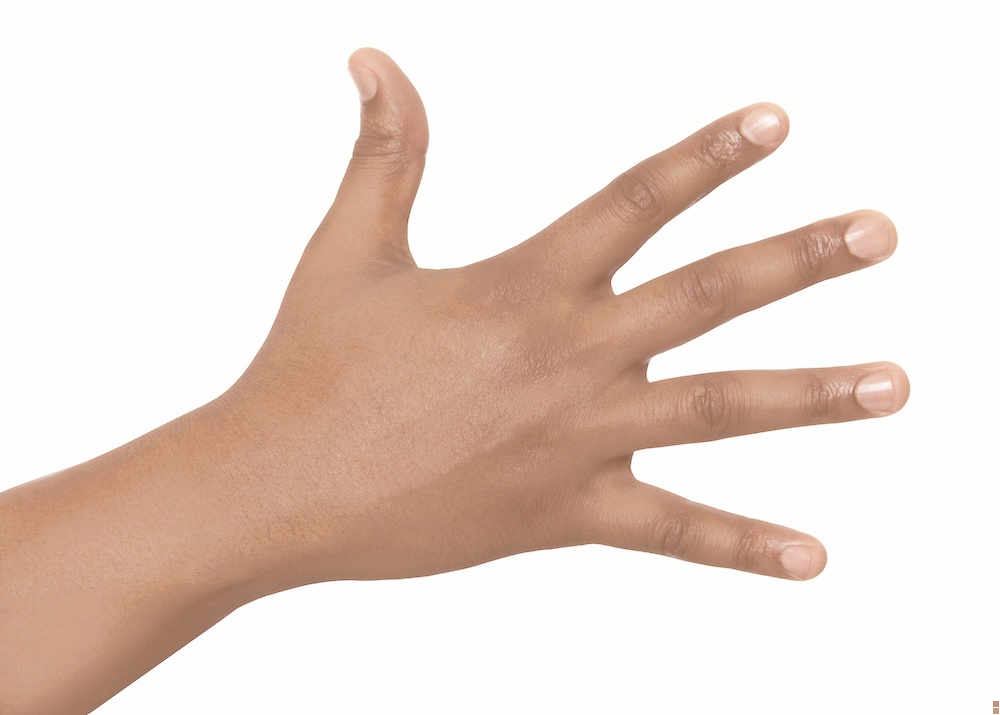
\includegraphics[width=\textwidth,height=\textheight,keepaspectratio]{../rc_test/outputs/20170517_proportional_corrected_test_alpha3/hand_dark_to_hand_light.jpg}
  \end{minipage} \\
    \hline  \ref{row:prop_correct_test_a3_hand_brown_to_hand_dark} &
  \begin{minipage}{.29\textwidth}
    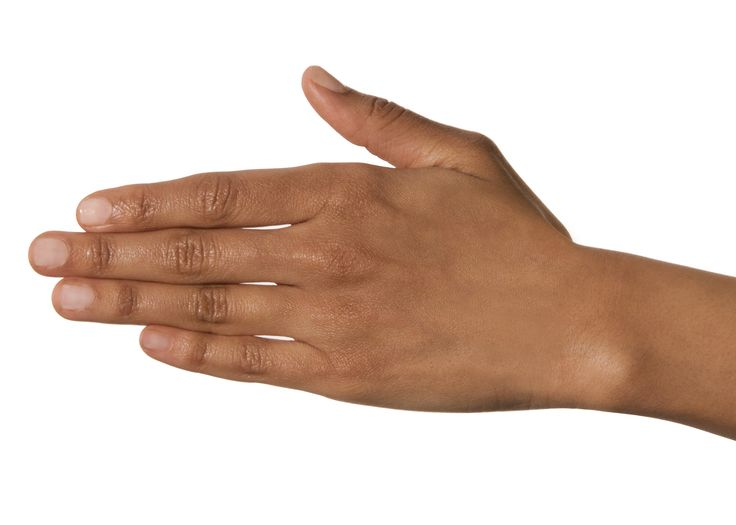
\includegraphics[width=\textwidth,height=\textheight,keepaspectratio]{../inputs/hand_brown.jpg}
  \end{minipage} & 
  \begin{minipage}{.29\textwidth}
    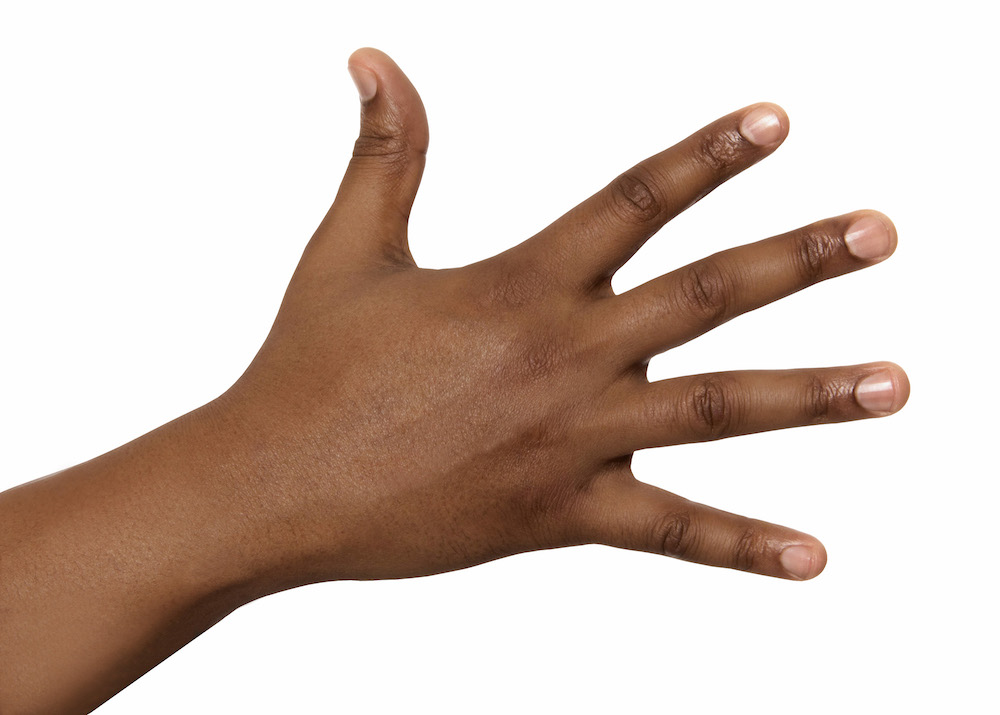
\includegraphics[width=\textwidth,height=\textheight,keepaspectratio]{../inputs/hand_dark.jpg}
  \end{minipage} & 
  \begin{minipage}{.29\textwidth}
    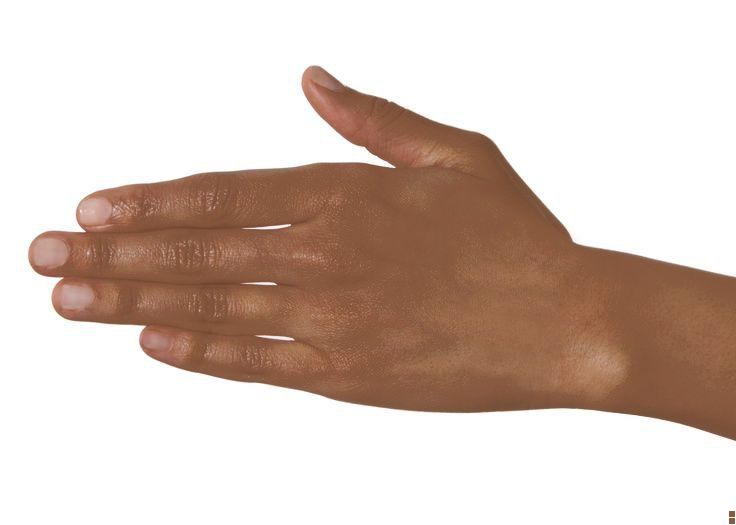
\includegraphics[width=\textwidth,height=\textheight,keepaspectratio]{../rc_test/outputs/20170517_proportional_corrected_test_alpha3/hand_brown_to_hand_dark.jpg}
  \end{minipage} \\
\hline  \ref{row:prop_correct_test_a3_hand_brown_to_hand_light} &
  \begin{minipage}{.29\textwidth}
    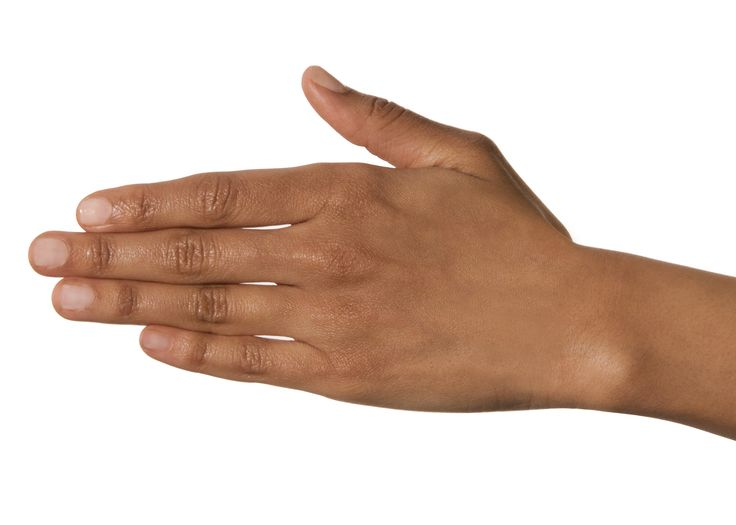
\includegraphics[width=\textwidth,height=\textheight,keepaspectratio]{../inputs/hand_brown.jpg}
  \end{minipage} & 
  \begin{minipage}{.29\textwidth}
    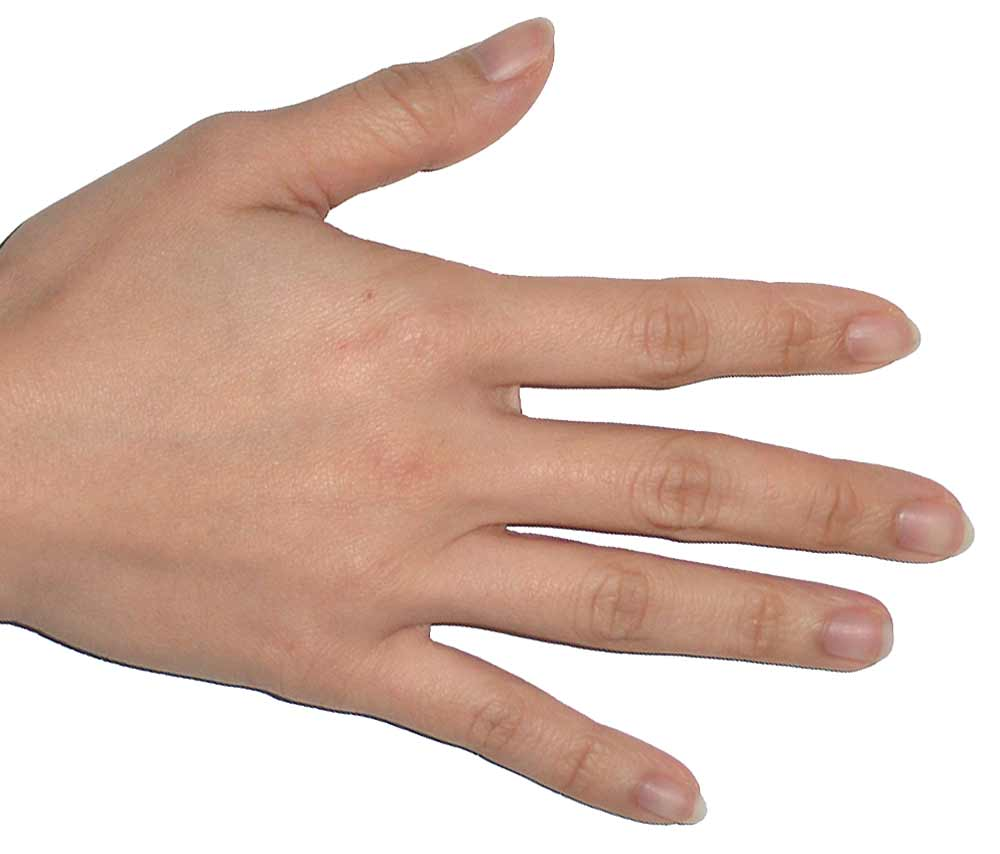
\includegraphics[width=\textwidth,height=\textheight,keepaspectratio]{../inputs/hand_light.jpg}
  \end{minipage} & 
  \begin{minipage}{.29\textwidth}
    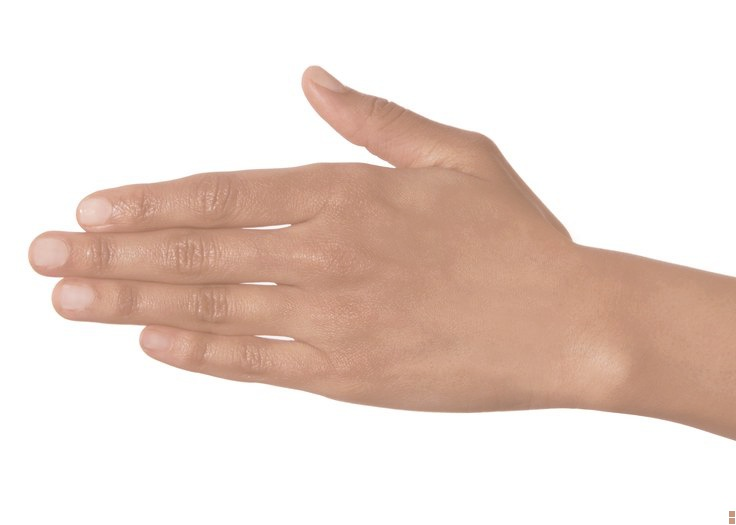
\includegraphics[width=\textwidth,height=\textheight,keepaspectratio]{../rc_test/outputs/20170517_proportional_corrected_test_alpha3/hand_brown_to_hand_light.jpg}
  \end{minipage} \\
  \hline  \ref{row:prop_correct_test_a3_hand_brown_to_hand_pale} &
  \begin{minipage}{.29\textwidth}
    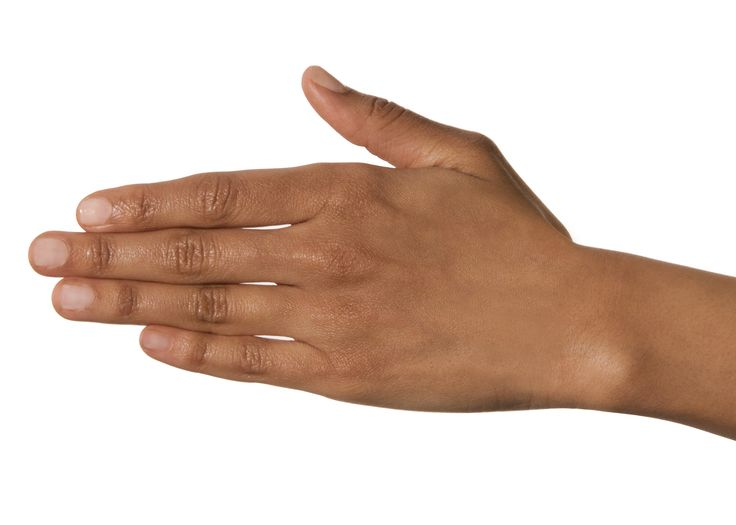
\includegraphics[width=\textwidth,height=\textheight,keepaspectratio]{../inputs/hand_brown.jpg}
  \end{minipage} & 
  \begin{minipage}{.29\textwidth}
    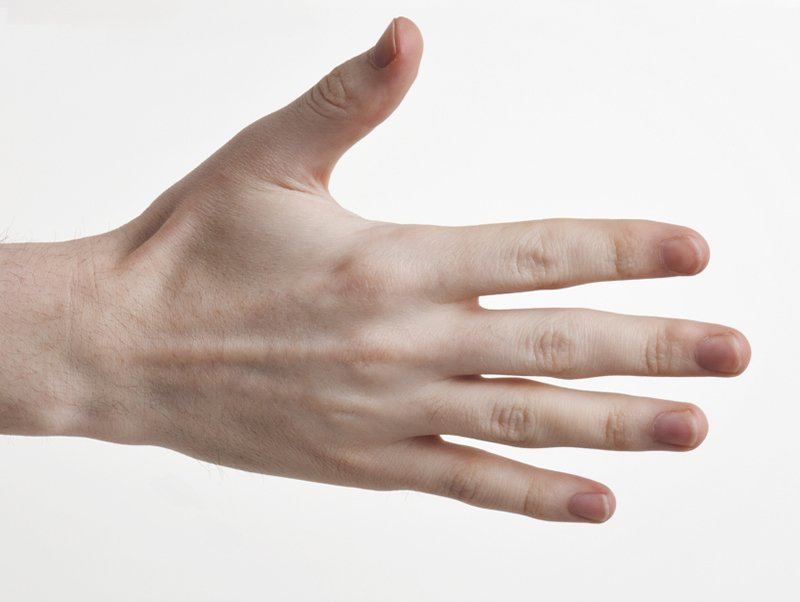
\includegraphics[width=\textwidth,height=\textheight,keepaspectratio]{../inputs/hand_pale.jpg}
  \end{minipage} & 
  \begin{minipage}{.29\textwidth}
    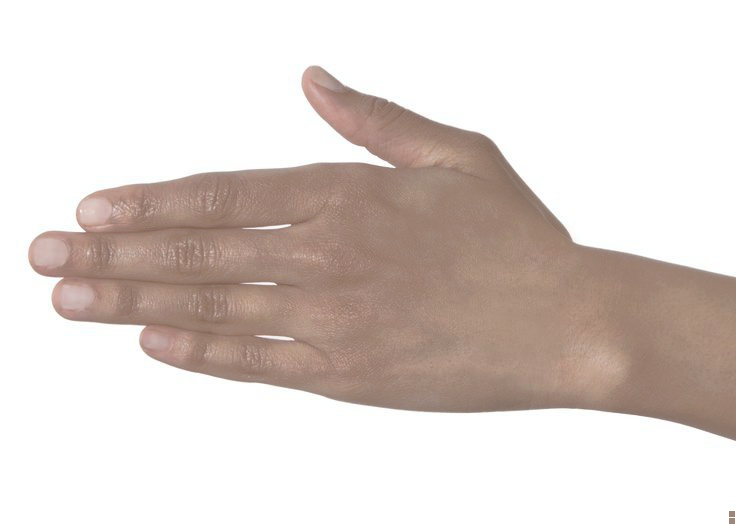
\includegraphics[width=\textwidth,height=\textheight,keepaspectratio]{../rc_test/outputs/20170517_proportional_corrected_test_alpha3/hand_brown_to_hand_pale.jpg}
  \end{minipage} \\
    \hline
\end{longtable}

\subsubsection*{Evaluation}
As show in Figure \ref{img:compare_dark_spot}, the dark spots and creases noted in Section \ref{sec:algo_prop_eval} are reduced.

\begin{figure}[H]
    \centering
    \begin{subfigure}[b]{0.40\textwidth}
        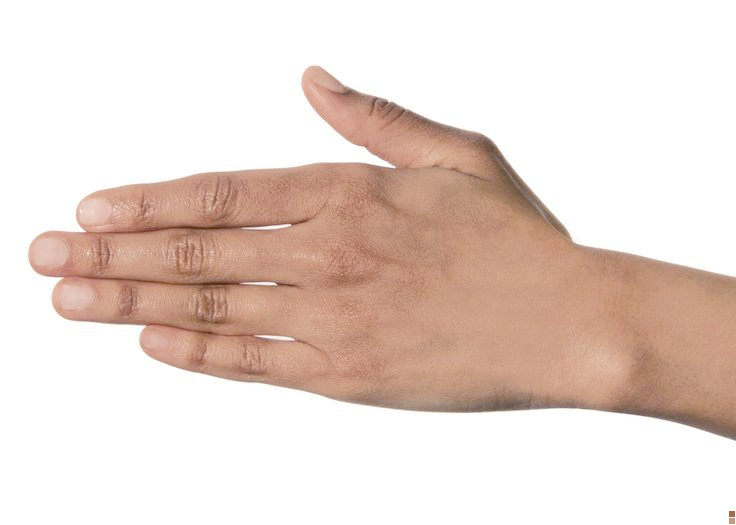
\includegraphics[width=\textwidth]{../rc_test/outputs/20170516_proportional_test/hand_brown_to_hand_light.jpg}
        \caption{Proportional adjustment algorithm (Equation \ref{eq:prop_algo})result}
    \end{subfigure}
    ~
    \begin{subfigure}[b]{0.40\textwidth}
        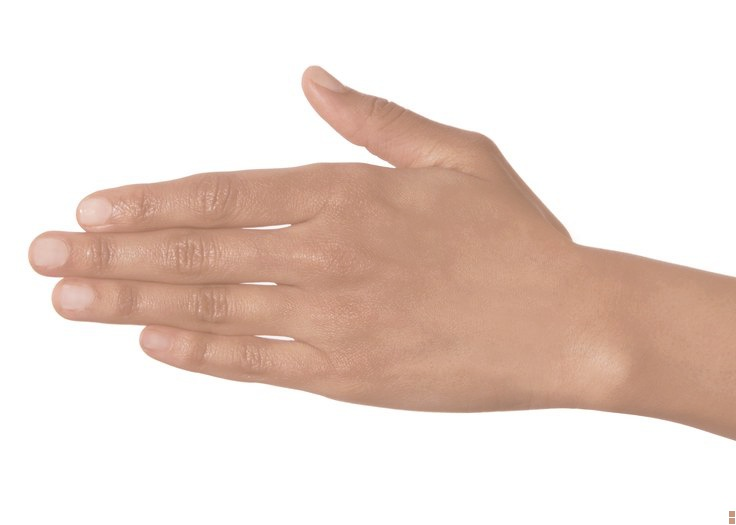
\includegraphics[width=\textwidth]{../rc_test/outputs/20170517_proportional_corrected_test_alpha3/hand_brown_to_hand_light.jpg}
        \caption{Proportional adjustment algorithm with correction (Equation \ref{eq:prop_corr_algo}) result}
    \end{subfigure}
    \caption{Comparison of algorithms \ref{eq:prop_algo} and \ref{eq:prop_corr_algo} results for transforming a mid-toned hand (Figure \ref{img:input_hands_1_brown}) to a light hand (Figure \ref{img:input_hands_1_light}).\label{img:compare_dark_spot}}
\end{figure}

However, we have noted that even for the more lower strength effect where $\alpha = 3$, this process brings back the problem of eliminating true black from the image, making the image appear once again to be without shadows (See Row \ref{row:prop_correct_test_a3_hand_dark_to_hand_brown} and \ref{row:prop_correct_test_a3_hand_brown_to_hand_light}). 

Also, it should be noted that for completeness, we performed this algorithm on all possible combinations of hand images, even though it was targeted at cases where the original image is of a skin tone darker than the new image. 

Interestingly, in a couple of cases of transformation from lighter skin tone to darker skin tone, the hand takes on a darker colour around joints in a similar manner to how a hand of dark skin tone is naturally coloured, though the algorithm was not intended for this purpose (See Row \ref{row:prop_correct_test_a3_hand_brown_to_hand_dark} as well as \ref{row:prop_correct_test_a3_hand_light_to_hand_dark}, \ref{row:prop_correct_test_a3_hand_light_to_hand_brown}). This is not always the case, however. Row \ref{row:prop_correct_test_a3_hand_pale_to_hand_dark} does not seem to exhibit this effect, possibly due to the different lighting of the hand in the image.